%
\section{Verifikation mit IntelliTest}

\emph{IntelliTests} generieren aus bestehendem Quellcode automatisch Tests, welche alle möglichen Pfade im Quelltext abdecken.~\cite{intellitest-correctness} Beim Versuch das Werkzeug auf C\# Essentials anzuwenden gab es Probleme mit dem Input. 

Das erste Problem bezieht sich auf die Herkunft. Die Klassen benötigen verschiedene Kontexte aus Visual Studio, um richtig initialisiert zu sein. Es ist leider nicht gelungen einen solchen validen Kontext innerhalb eines Tests zu erzeugen.

Das zweite Problem entsteht beim erzeugen von IntelliTests aus UnitTests. IntelliTest unterstützt zwar diese Funktion, jedoch bricht der Testlauf nach einigen Sekunden ab, weil die Anzahl der möglichen Eingaben zu groß ist.

Um dennoch die Arbeitsweise von IntelliTest zu veranschaulichen im folgenden ein Beispiel. In Listing~\ref{lst:calculator} sieht man die Klasse \texttt{Calculator} mit ihrer Methode \texttt{Add}. Um einen mögliches Fehlverhalten zu simulieren, gibt diese Methode, wann immer die beiden Summanden gleich sind, den zweiten Summanden zurück.

\begin{lstlisting}[caption={Klasse \texttt{Calculator}},
label=lst:calculator]
class Calculator
{
	public int Add(int a, int b)
	{
		if (a == b && a > 20) return b;
		
		return a + b;
	}
}
\end{lstlisting}

\begin{lstlisting}[caption={Test \texttt{Calculator}},
label=lst:calculator-test]
[PexClass(typeof(Calculator))]
[PexAllowedExceptionFromTypeUnderTest(
	typeof(InvalidOperationException))]
[PexAllowedExceptionFromTypeUnderTest(
	typeof(ArgumentException), AcceptExceptionSubtypes = true)]
[TestClass]
public partial class CalculatorTest
{
	/// <summary>Test stub for Add(Int32, Int32)</summary>
	[PexMethod]
	internal int AddTest(
	[PexAssumeUnderTest]Calculator target,
	int a,
	int b
	)
	{
		int result = target.Add(a, b);
		PexAssert.AreEqual(a+b, result);
		return result;
	}
}
\end{lstlisting}

Der generierte Testfall ist in Listing~\ref{lst:calculator-test} dargestellt. Beim Ausführen des Tests stellt IntelliTest korrekt fest, dass die Eingaben a = 21 und b = 21 zu einem falschen Ergebnis führen. In Abbildung~\ref{fig:intellitest} ist die entsprechende Ausgabe zu sehen.

\begin{figure}[!ht]
	\centering
	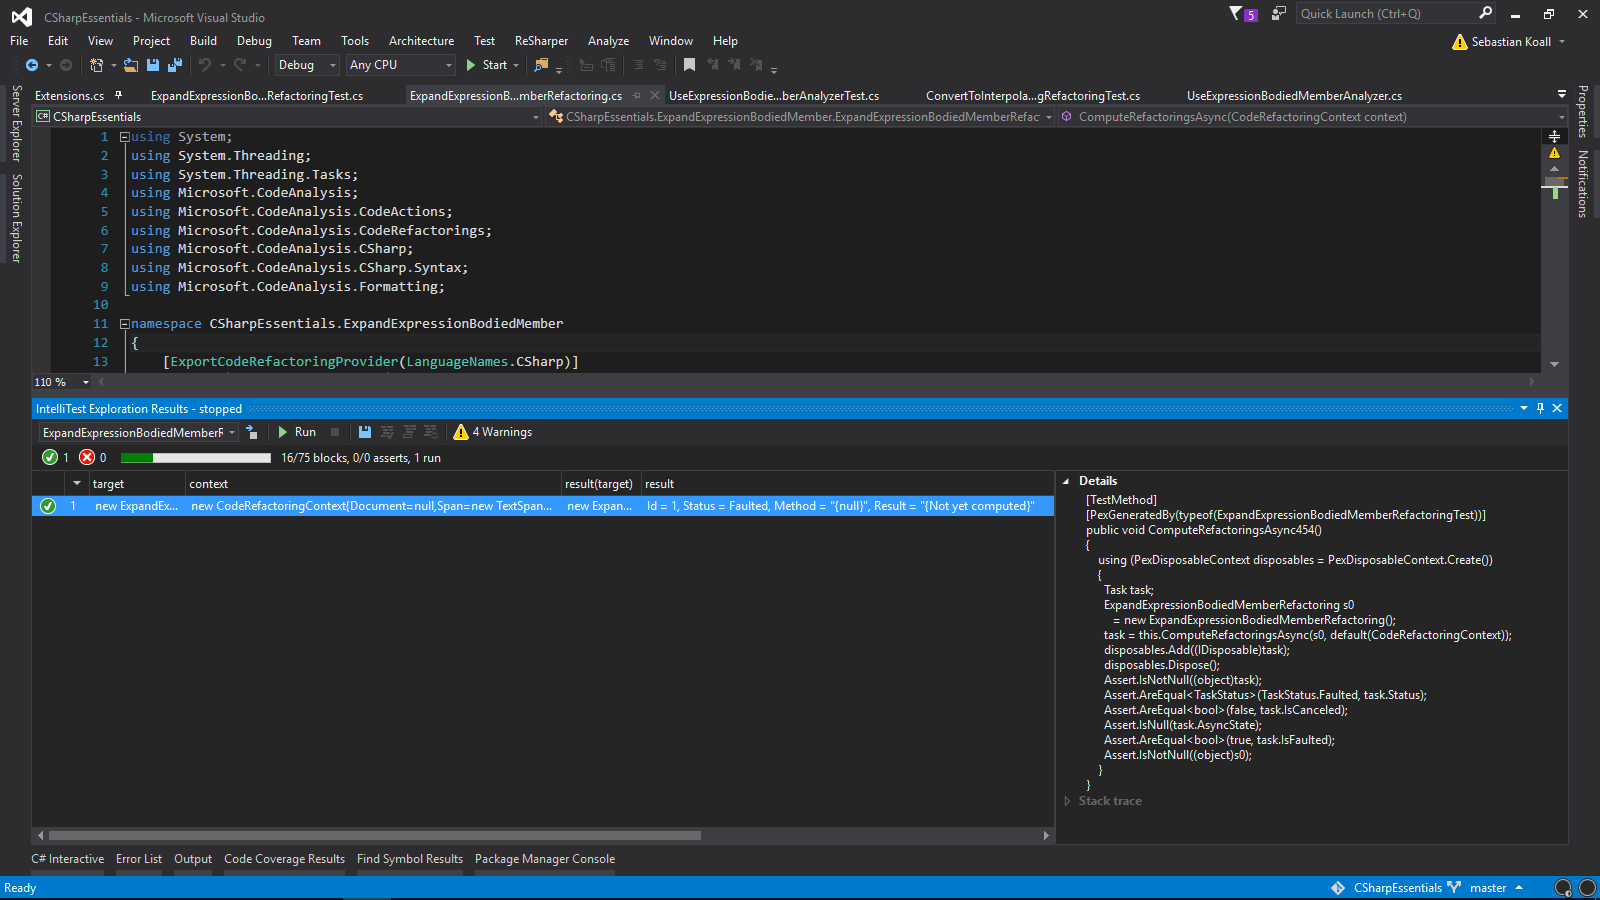
\includegraphics[width=0.9\textwidth]{images/intellitest.png}
	\caption{IntelliTest Ausgabe der Methode \texttt{Add}}
	\vspace{0.1cm}
	IntelliTest findet den zufälligen Fehler bei Gleichheit über 20
	\label{fig:intellitest}
\end{figure}

Zusammenfassend lässt sich feststellen, dass IntelliTest ein interessantes Werkzeug ist, sich jedoch leider bisher nicht auf jede beliebige Eingabe anwenden lässt.